% Mid-term evaluation slides. Build (twice): xelatex slides.tex
\documentclass[aspectratio=169,11pt]{beamer}
\usetheme[progressbar=frametitle,numbering=fraction]{metropolis}

\usepackage{booktabs}
\usepackage{tabularx}
\usepackage{array}
\usepackage{graphicx}
\usepackage{tikz}
\usetikzlibrary{arrows.meta,positioning,calc}
\graphicspath{{fig/}}

\definecolor{done}{HTML}{1A9850}
\definecolor{next}{HTML}{9E9E9E}
\definecolor{built}{HTML}{D7301F}
\definecolor{accent}{HTML}{2C7FB8}
\setbeamercolor{alerted text}{fg=accent}
\newcommand{\hl}[1]{\alert{\textbf{#1}}}
\newcolumntype{L}[1]{>{\raggedright\arraybackslash}p{#1}}
\newcolumntype{Y}{>{\raggedright\arraybackslash}X}
\setlength{\leftmargini}{1.2em}

\title{GIS-Based Land Suitability Analysis for Urban Development\\using Land Use Land Cover}
\subtitle{Mid-term evaluation}
\author{Harsh Chattar (22CS30028) \quad Abhinav (22CS30005)}
\institute{CS60111 Geographical Information Systems}
\date{6 October 2026}

\begin{document}

% ------------------------------------------------------------------ 1
\maketitle

% ------------------------------------------------------------------ 2
\begin{frame}{Problem and goal}
  \small
  \begin{columns}[T]
    \begin{column}{0.55\textwidth}
      \textbf{Problem}
      \begin{itemize}
        \item Cities like Bengaluru grow fast into surrounding land.
              \emph{Where} can new development reasonably go?
        \item Classic GIS suitability (weighted overlay / AHP) relies on
              \hl{hand-set weights} and is rarely checked against real growth.
      \end{itemize}
      \vspace{0.5em}
      \textbf{Goal}
      \begin{itemize}
        \item A \hl{data-driven} suitability map from land use / land cover,
              terrain, roads and existing buildings, fully in \textbf{Python}.
        \item \hl{Validated} against growth that actually happened.
      \end{itemize}
    \end{column}
    \begin{column}{0.42\textwidth}
      \textbf{Questions}
      \begin{enumerate}
        \item Which land is \textcolor{built}{\textbf{built-up}},
              \textcolor{done}{\textbf{forest}} or \textbf{usable}?
        \item Given a building at \textbf{A}, where are locations \textbf{B}
              with \emph{similar surroundings}?
        \item Does our ranking predict where the city \emph{actually} grew?
      \end{enumerate}
    \end{column}
  \end{columns}
\end{frame}

% ------------------------------------------------------------------ 3
\begin{frame}{Approach}
  \centering
  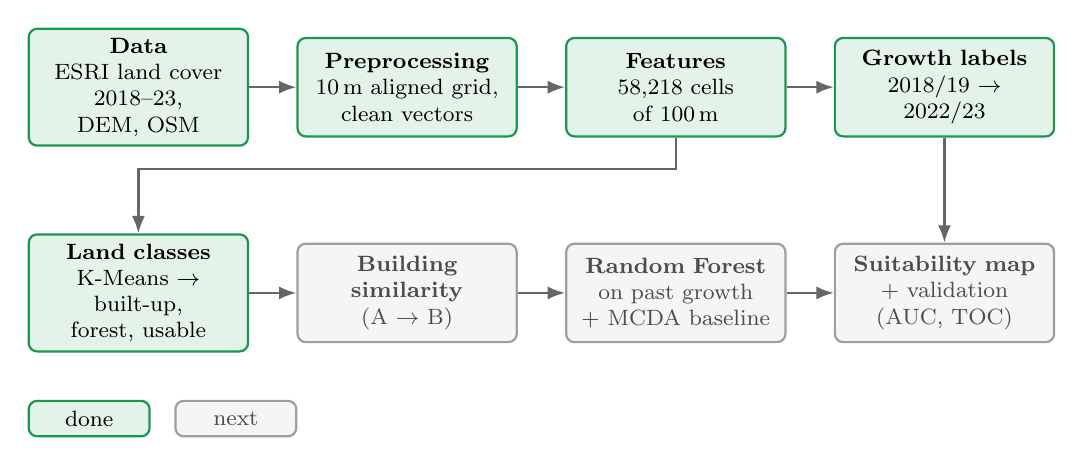
\begin{tikzpicture}[
      box/.style={draw, rounded corners=3pt, align=center, font=\footnotesize,
                  minimum height=1.25cm, text width=2.55cm, line width=0.8pt},
      d/.style={box, draw=done, fill=done!12},
      n/.style={box, draw=next, fill=next!10, text=black!70},
      arr/.style={-{Latex[length=2.2mm]}, line width=0.8pt, black!60},
      node distance=0.5cm and 0.6cm]
    \node[d] (data) {\textbf{Data}\\ESRI land cover\\2018--23, DEM, OSM};
    \node[d, right=of data] (prep) {\textbf{Preprocessing}\\10\,m aligned grid,\\clean vectors};
    \node[d, right=of prep] (feat) {\textbf{Features}\\58{,}218 cells\\of 100\,m};
    \node[d, right=of feat] (lab) {\textbf{Growth labels}\\2018/19 $\rightarrow$ 2022/23};
    \node[d, below=1.1cm of data] (cls) {\textbf{Land classes}\\K-Means $\rightarrow$ built-up,\\forest, usable};
    \node[n, right=of cls] (sim) {\textbf{Building similarity}\\(A $\rightarrow$ B)};
    \node[n, right=of sim] (rf) {\textbf{Random Forest}\\on past growth\\+ MCDA baseline};
    \node[n, right=of rf] (val) {\textbf{Suitability map}\\+ validation\\(AUC, TOC)};
    \draw[arr] (data) -- (prep);
    \draw[arr] (prep) -- (feat);
    \draw[arr] (feat) -- (lab);
    \draw[arr] (feat.south) -- ++(0,-0.4) -| (cls.north);
    \draw[arr] (cls) -- (sim);
    \draw[arr] (sim) -- (rf);
    \draw[arr] (rf) -- (val);
    \draw[arr] (lab.south) -- (val.north);
    \node[d, minimum height=0.45cm, text width=1.3cm, below=0.6cm of cls.south west, anchor=north west] (k1) {done};
    \node[n, minimum height=0.45cm, text width=1.3cm, right=0.3cm of k1] (k2) {next};
  \end{tikzpicture}
\end{frame}

% ------------------------------------------------------------------ 4
\begin{frame}{Key idea: building similarity, checked against real growth}
  \begin{columns}[T]
    \begin{column}{0.47\textwidth}
      \centering
      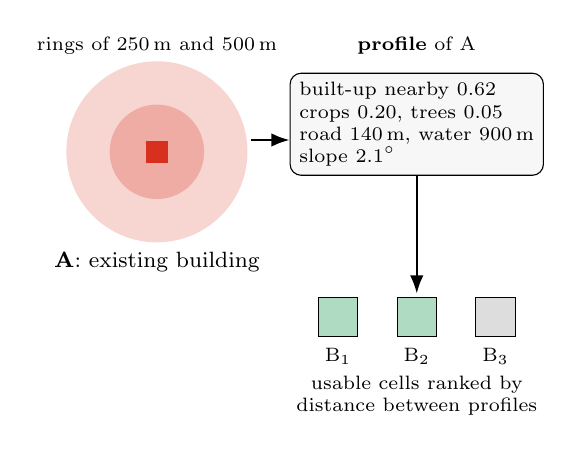
\begin{tikzpicture}[every node/.style={font=\scriptsize}]
        \fill[built!20] (0,0) circle (1.15);
        \fill[built!40] (0,0) circle (0.6);
        \fill[built] (-0.14,-0.14) rectangle (0.14,0.14);
        \node[font=\footnotesize] at (0,-1.4) {\textbf{A}: existing building};
        \node at (0,1.35) {rings of 250\,m and 500\,m};
        \node[draw, rounded corners, align=left, fill=black!3] (p) at (3.3,0.35)
          {built-up nearby 0.62\\crops 0.20, trees 0.05\\road 140\,m, water 900\,m\\slope 2.1$^\circ$};
        \node at (3.3,1.35) {\textbf{profile} of A};
        \draw[-{Latex}, thick] (1.2,0.15) -- (p.west |- 0,0.15);
        \foreach \x/\lbl/\c in {2.3/B$_1$/done, 3.3/B$_2$/done, 4.3/B$_3$/next} {
          \draw[fill=\c!35] (\x-0.25,-2.35) rectangle (\x+0.25,-1.85);
          \node at (\x,-2.6) {\lbl};
        }
        \draw[-{Latex}, thick] (p.south) -- (3.3,-1.8);
        \node[align=center] at (3.3,-3.1) {usable cells ranked by\\distance between profiles};
      \end{tikzpicture}
    \end{column}
    \begin{column}{0.51\textwidth}
      \small
      \textbf{How we test it: travel back to 2018}
      \begin{itemize}
        \item Rebuild everything \hl{as of 2018}: land cover 2018/19, OpenStreetMap
              \emph{as it was on 1 Jan 2018}.
        \item Rank the land that was still non-built.
        \item Compare with cells that became built in \hl{both 2022 and 2023}.
      \end{itemize}
      \vspace{0.4em}
      \textbf{No information leaks}
      \begin{itemize}
        \item Models see only a cell's \emph{surroundings}, never its own land cover.
        \item Today's OSM has \hl{over twice the roads} of 2018: using it would leak future growth.
      \end{itemize}
    \end{column}
  \end{columns}
\end{frame}

% ------------------------------------------------------------------ 5
\begin{frame}{Literature: the 8 most relevant studies}
  \vspace{-0.6em}
  \scriptsize
  \renewcommand{\arraystretch}{1.0}
  \setlength{\tabcolsep}{4pt}
  \begin{tabularx}{\textwidth}{@{}L{2.75cm} Y L{2.8cm} L{3.9cm}@{}}
    \toprule
    \textbf{Study} & \textbf{Method} & \textbf{Validation} & \textbf{Relevance to us} \\
    \midrule
    Li et al.\ 2024, Yulin, China & Random Forest, built-up vs protected land & random split: AUC 0.99 & closest work; own-cell land use inflates AUC \\
    Ahmadlou et al.\ 2016, Rasht, Iran & Random Forest, Landsat 1985--2015 & later change: AUC 0.82, TOC & same test-on-later-growth design \\
    Wang et al.\ 2021, Luoyang, China & MaxEnt (presence-only) + CA & 2009$\rightarrow$2018: Kappa 0.78 & presence-only, like similarity \\
    Liu et al.\ 2017, FLUS, China & neural-net suitability + CA & 2000$\rightarrow$2010 vs actual & standard learned-suitability model \\
    Pijanowski et al.\ 2002, LTM, USA & neural net, distances + neighbourhood & 46\,\% of changes & ancestor of our neighbourhood features \\
    Malczewski 2004 & review of GIS multi-criteria methods & -- & our MCDA baseline; subjective weights \\
    Roberts et al.\ 2017 & blocked vs random cross-validation & random CV too optimistic & spatial blocks in our validation \\
    Venter et al.\ 2022 & Esri vs WorldCover vs Dynamic World & Esri most accurate (75\,\%) & why ESRI; it over-predicts scrub \\
    \bottomrule
  \end{tabularx}
  \vspace{0.3em}

  \footnotesize\textbf{Gap:} none searches for places like a \emph{specific building}; few test on \emph{later} growth.
\end{frame}

% ------------------------------------------------------------------ 6
\begin{frame}{Study area: Bengaluru South}
  \begin{columns}[T]
    \begin{column}{0.53\textwidth}
      \vspace{-0.5em}
      \small 14 candidate areas compared on land cover, growth and OSM history:\\[0.2em]
      \scriptsize
      \begin{tabular}{@{}lrrr@{}}
        \toprule
        Area & Growth\textsuperscript{*} & Trees & OSM buildings 2018 \\
        \midrule
        Ranchi & 10.1\,\% & 15.5\,\% & 558 \\
        Hyderabad West & 9.9\,\% & 14.3\,\% & 191k \\
        \textbf{Bengaluru South} & \textbf{8.4\,\%} & \textbf{19.2\,\%} & \textbf{151k} \\
        Gurugram & 8.0\,\% & 13.5\,\% & 123k \\
        Pune West & 7.1\,\% & 18.3\,\% & 118k \\
        Coimbatore & 6.9\,\% & 23.8\,\% & 736 \\
        \bottomrule
      \end{tabular}\\[0.15em]
      \tiny\textsuperscript{*} share of 2018 non-built land that became built in both 2022 and 2023\\[0.2em]
      \footnotesize
      \begin{itemize}
        \item 582\,km$^2$: Electronic City, Hosur Road, Kanakapura Road.
        \item Strong growth, a clear forest block (\hl{Bannerghatta NP}).
        \item OSM already well mapped \hl{in 2018}, as the test needs.
      \end{itemize}
    \end{column}
    \begin{column}{0.45\textwidth}
      \centering
      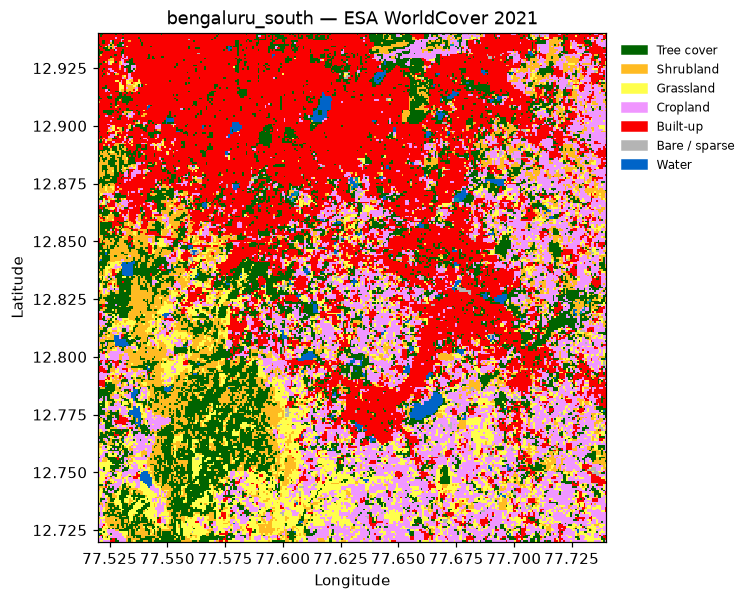
\includegraphics[height=0.8\textheight]{study_area.png}
    \end{column}
  \end{columns}
\end{frame}

% ------------------------------------------------------------------ 7
\begin{frame}{Data}
  \begin{columns}[T]
    \begin{column}{0.4\textwidth}
      \scriptsize
      \renewcommand{\arraystretch}{1.15}
      \begin{tabularx}{\textwidth}{@{}Y L{1.5cm}@{}}
        \toprule
        \textbf{Dataset} & \textbf{Years} \\
        \midrule
        \textbf{ESRI land use / land cover}, 10\,m: land cover, land classes, growth labels & 2018--2023, every year \\
        \textbf{ESA WorldCover}, 10\,m: independent cross-check & 2021 \\
        \textbf{Copernicus DEM}, 30\,m: elevation, slope & static \\
        \textbf{OpenStreetMap}: roads, water, buildings, protected areas & 1 Jan 2018 + today \\
        \bottomrule
      \end{tabularx}\\[0.6em]
      \small Today's OSM has \hl{2.1$\times$ the roads} of 2018, so the 2018 test must use the
      2018 snapshot.
    \end{column}
    \begin{column}{0.58\textwidth}
      \centering
      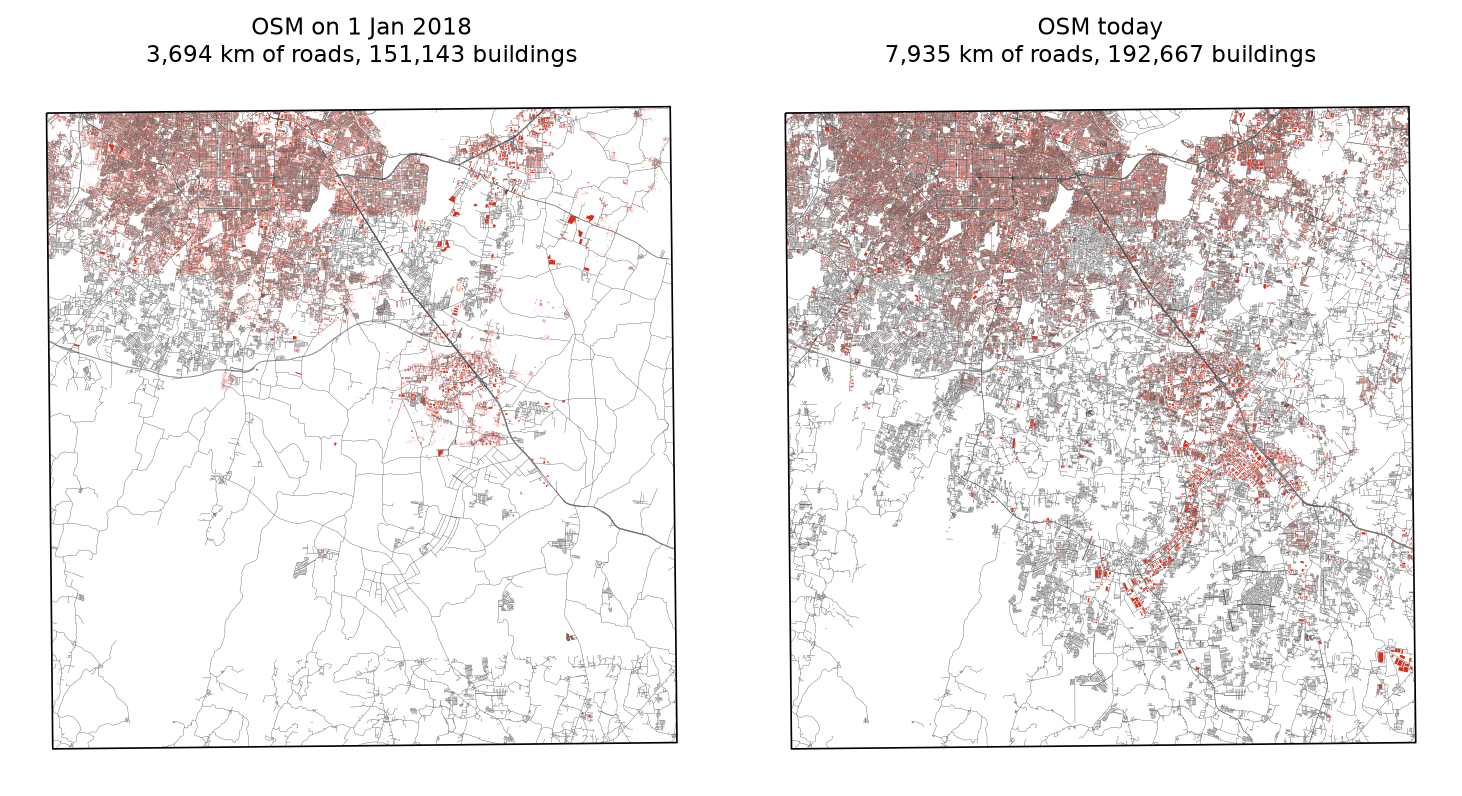
\includegraphics[width=\textwidth]{osm_2018_vs_now.png}\\
      \scriptsize OSM inside the study area (drivable roads, buildings)
    \end{column}
  \end{columns}
\end{frame}

% ------------------------------------------------------------------ 8
\begin{frame}{Analysis grid and growth labels}
  \begin{columns}[T]
    \begin{column}{0.52\textwidth}
      \small
      \textbf{Grid:} \hl{58{,}218 cells} of 100\,m on the 10\,m land-cover pixels.\\
      \textbf{Per cell:} land-cover shares (own cell and 250 / 500\,m rings), elevation, slope,
      distance to roads / water / built-up, road density.\\[0.5em]
      \textbf{Growth labels}, two years at each end to ignore classifier noise:\\[0.2em]
      \scriptsize
      \begin{tabular}{@{}lr@{}}
        \toprule
        Candidate: non-built in 2018 \emph{and} 2019 & 15{,}658 \\
        \quad grew: built in 2022 \emph{and} 2023 & \textbf{1{,}125} \\
        \quad stayed non-built & 11{,}652 \\
        \quad partly grown (left out) & 2{,}881 \\
        Excluded: water, slope $>15^\circ$, protected & 6{,}253 \\
        \bottomrule
      \end{tabular}\\[0.3em]
      \small Growth rate \hl{8.8\,\%}; 1{,}034 grown cells are next to existing
      development, only \hl{91} are isolated.
    \end{column}
    \begin{column}{0.46\textwidth}
      \centering
      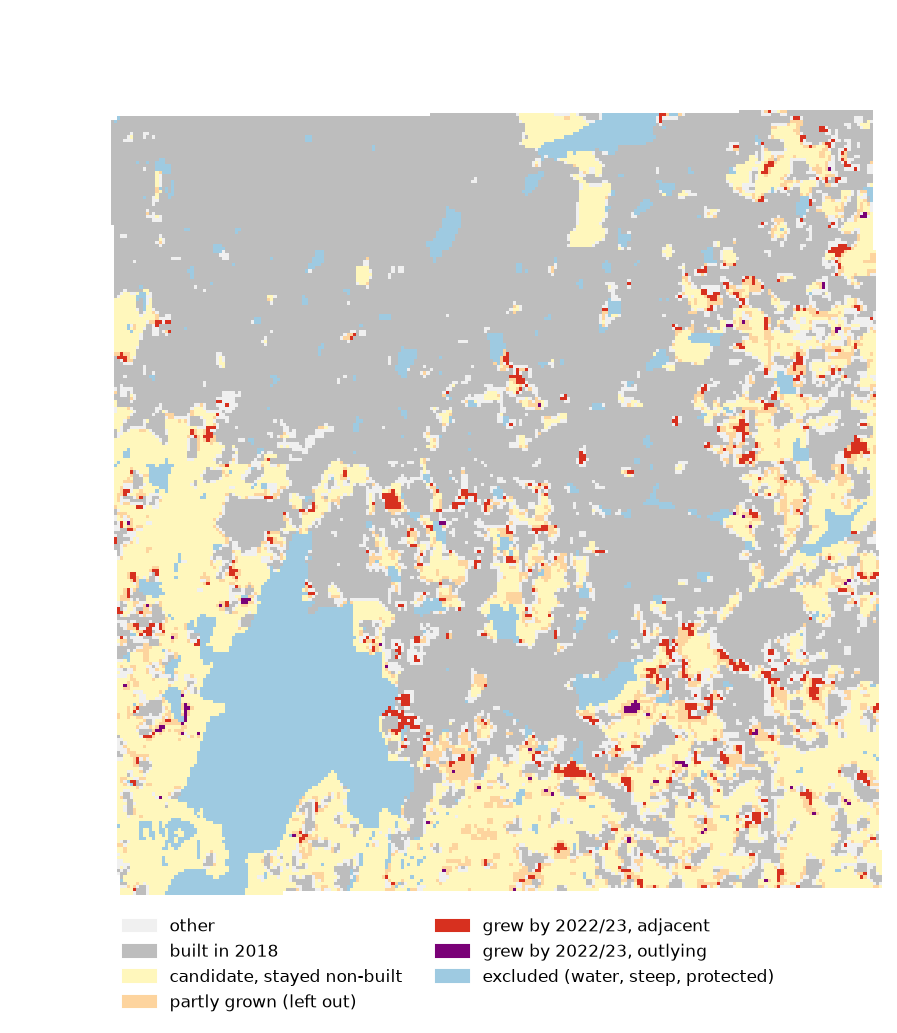
\includegraphics[height=0.82\textheight]{growth_labels.png}
    \end{column}
  \end{columns}
\end{frame}

% ------------------------------------------------------------------ 9
\begin{frame}{Land classification: clustering}
  \begin{columns}[T]
    \begin{column}{0.36\textwidth}
      \small
      \begin{itemize}
        \item Inputs: shares of built-up, trees, crops, rangeland, water + elevation, slope.
        \item K-Means vs Gaussian mixture, $k = 3 \dots 10$.
        \item \hl{K-Means, $k = 7$}: silhouette 0.61 (mixture $\le$ 0.36).
        \item Rules map clusters to classes; \emph{steep} rangeland = forest
              (Bannerghatta hills).
        \item Water, steep and protected cells are \textbf{excluded}.
      \end{itemize}
    \end{column}
    \begin{column}{0.62\textwidth}
      \centering
      \vspace{0.3em}
      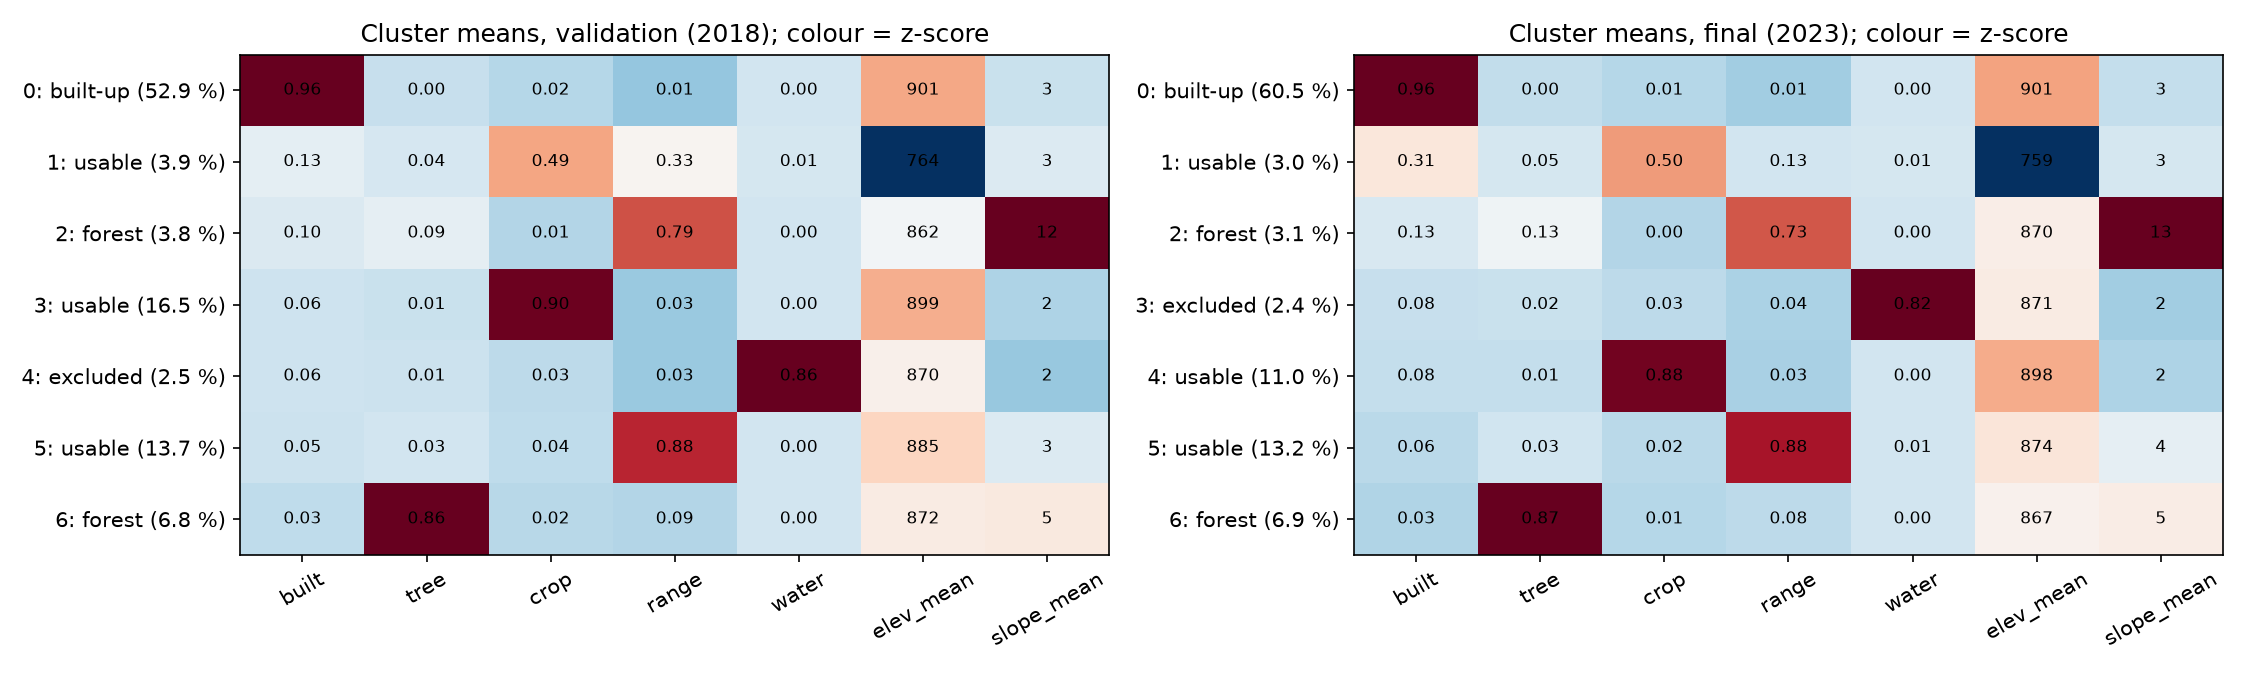
\includegraphics[width=\textwidth,trim={545bp 0 0 0},clip]{p5_cluster_profiles.png}\\
      \scriptsize Mean of each input per cluster, 2023 (colour = z-score)
    \end{column}
  \end{columns}
\end{frame}

% ------------------------------------------------------------------ 10
\begin{frame}{Land classification: results}
  \begin{columns}[T]
    \begin{column}{0.68\textwidth}
      \centering
      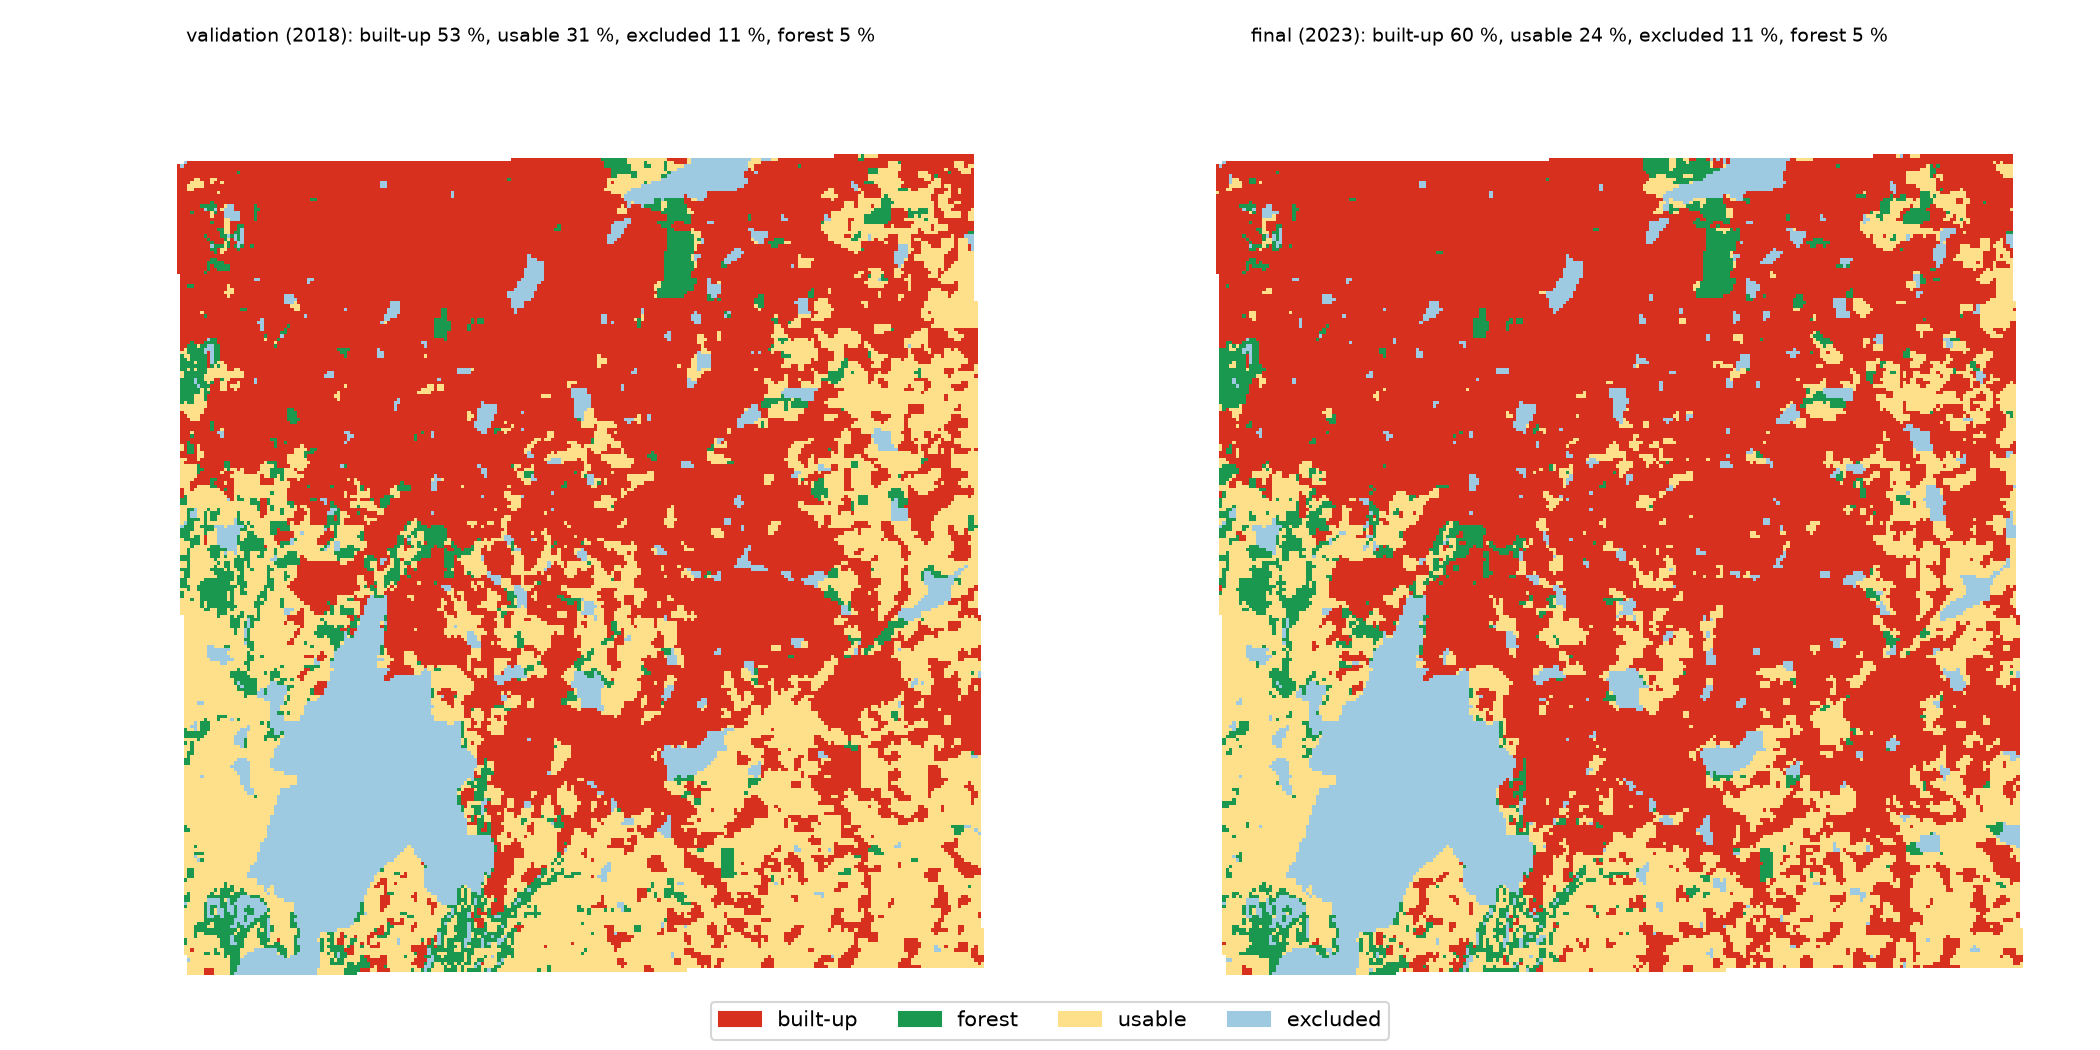
\includegraphics[width=\textwidth]{p5_class_maps.png}
    \end{column}
    \begin{column}{0.3\textwidth}
      \small
      \textbf{2018 $\rightarrow$ 2023}
      \begin{itemize}
        \item \textcolor{built}{\textbf{Built-up}}: 53\,\% $\rightarrow$ \textbf{60\,\%}
        \item Usable: 31\,\% $\rightarrow$ 24\,\%
        \item Forest 5\,\%, excluded 11\,\%
      \end{itemize}
      \textbf{Agreement} (land cells)
      \begin{itemize}
        \item ESRI: \hl{96.6\,\%}
        \item WorldCover: 64--71\,\%; the two products disagree
      \end{itemize}
      \textbf{Satellite check}: 4 of 5 random cells clearly right
    \end{column}
  \end{columns}
\end{frame}

% ------------------------------------------------------------------ 11
\begin{frame}{Next steps and challenges}
  \small
  \begin{columns}[T]
    \begin{column}{0.53\textwidth}
      \textbf{Next}
      \begin{enumerate}
        \item \textbf{Building similarity}: query A $\rightarrow$ B, and a score for
              every usable cell.
        \item \textbf{Random Forest} trained on 2018 $\rightarrow$ 2020/21 growth.
        \item \textbf{MCDA / AHP} weighted-overlay baseline.
        \item \textbf{Validation} on 2022/23 growth: ROC-AUC, TOC, lift;
              adjacent vs isolated growth.
        \item Final \textbf{suitability map} (S1--S3 / N) and candidate sites.
      \end{enumerate}
    \end{column}
    \begin{column}{0.45\textwidth}
      \textbf{Challenges}
      \begin{itemize}
        \item \hl{Distance to existing built-up} alone scores AUC $\approx$ 0.75
              in a pilot test: the bar to beat.
        \item ESRI's built-up class is broad on the urban fringe.
        \item Isolated growth is rare (91 cells), so hard to predict.
        \item Keeping today's data out of the 2018 test.
      \end{itemize}
    \end{column}
  \end{columns}
\end{frame}

% ------------------------------------------------------------------ 12
\begin{frame}[standout]
  Thank you\\[0.5em]
  \normalsize Questions?
\end{frame}

% ------------------------------------------------------------------ backup
\appendix

\begin{frame}{Backup: choosing $k$}
  \centering
  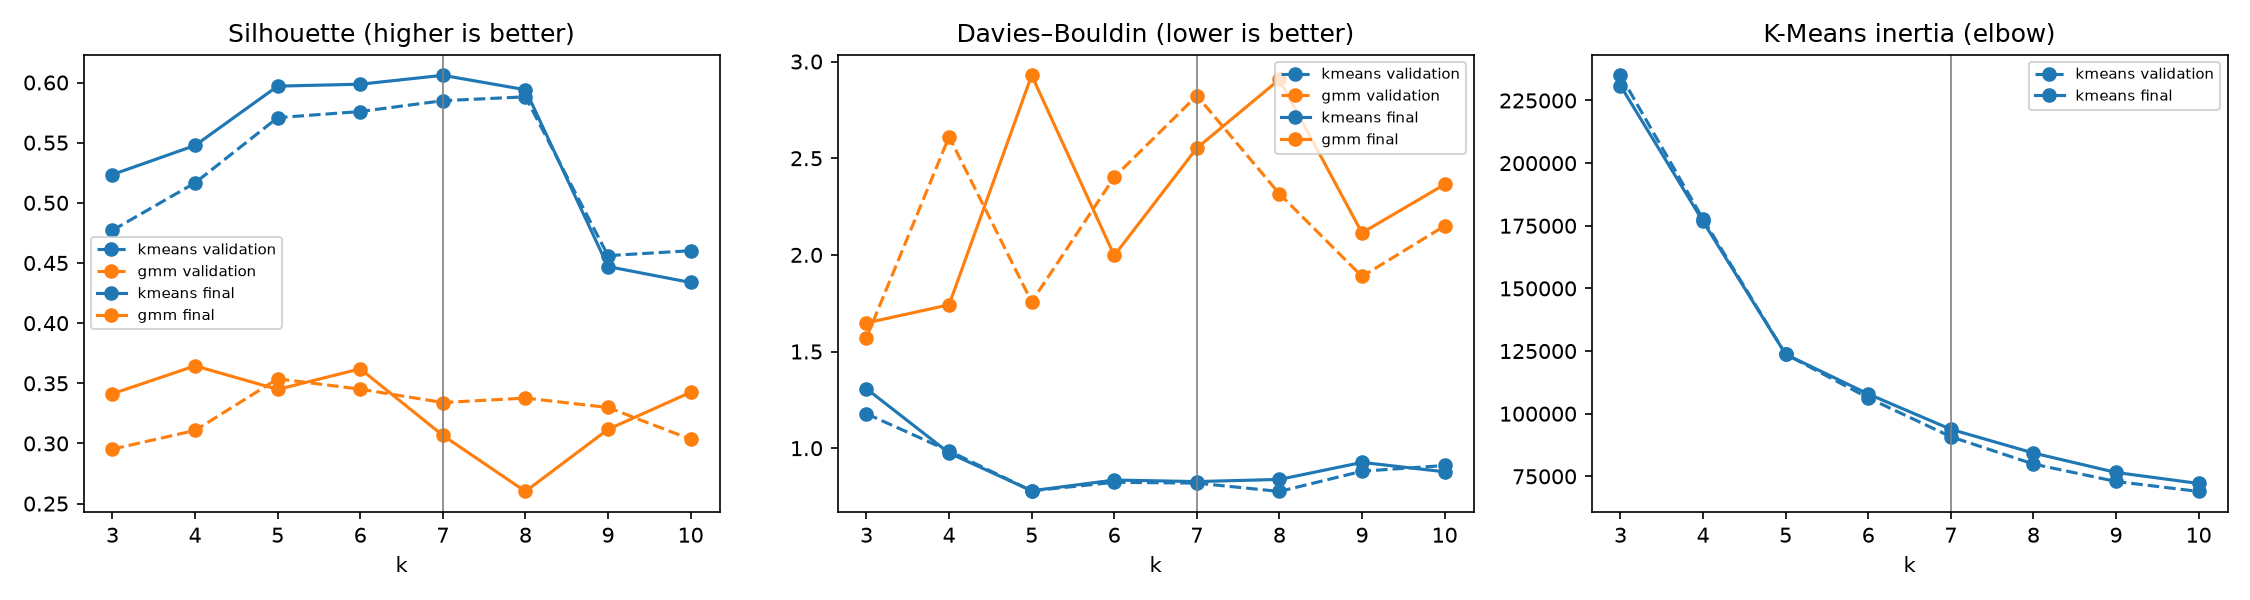
\includegraphics[width=\textwidth]{p5_k_scan.png}\\[0.3em]
  \small K-Means silhouette plateaus at $k = 5$--$8$ and drops at $k = 9$; $k = 7$ adds two
  interpretable clusters (steep rangeland, low western valley) in both years.
\end{frame}

\begin{frame}{Backup: satellite check of the land classes}
  \centering
  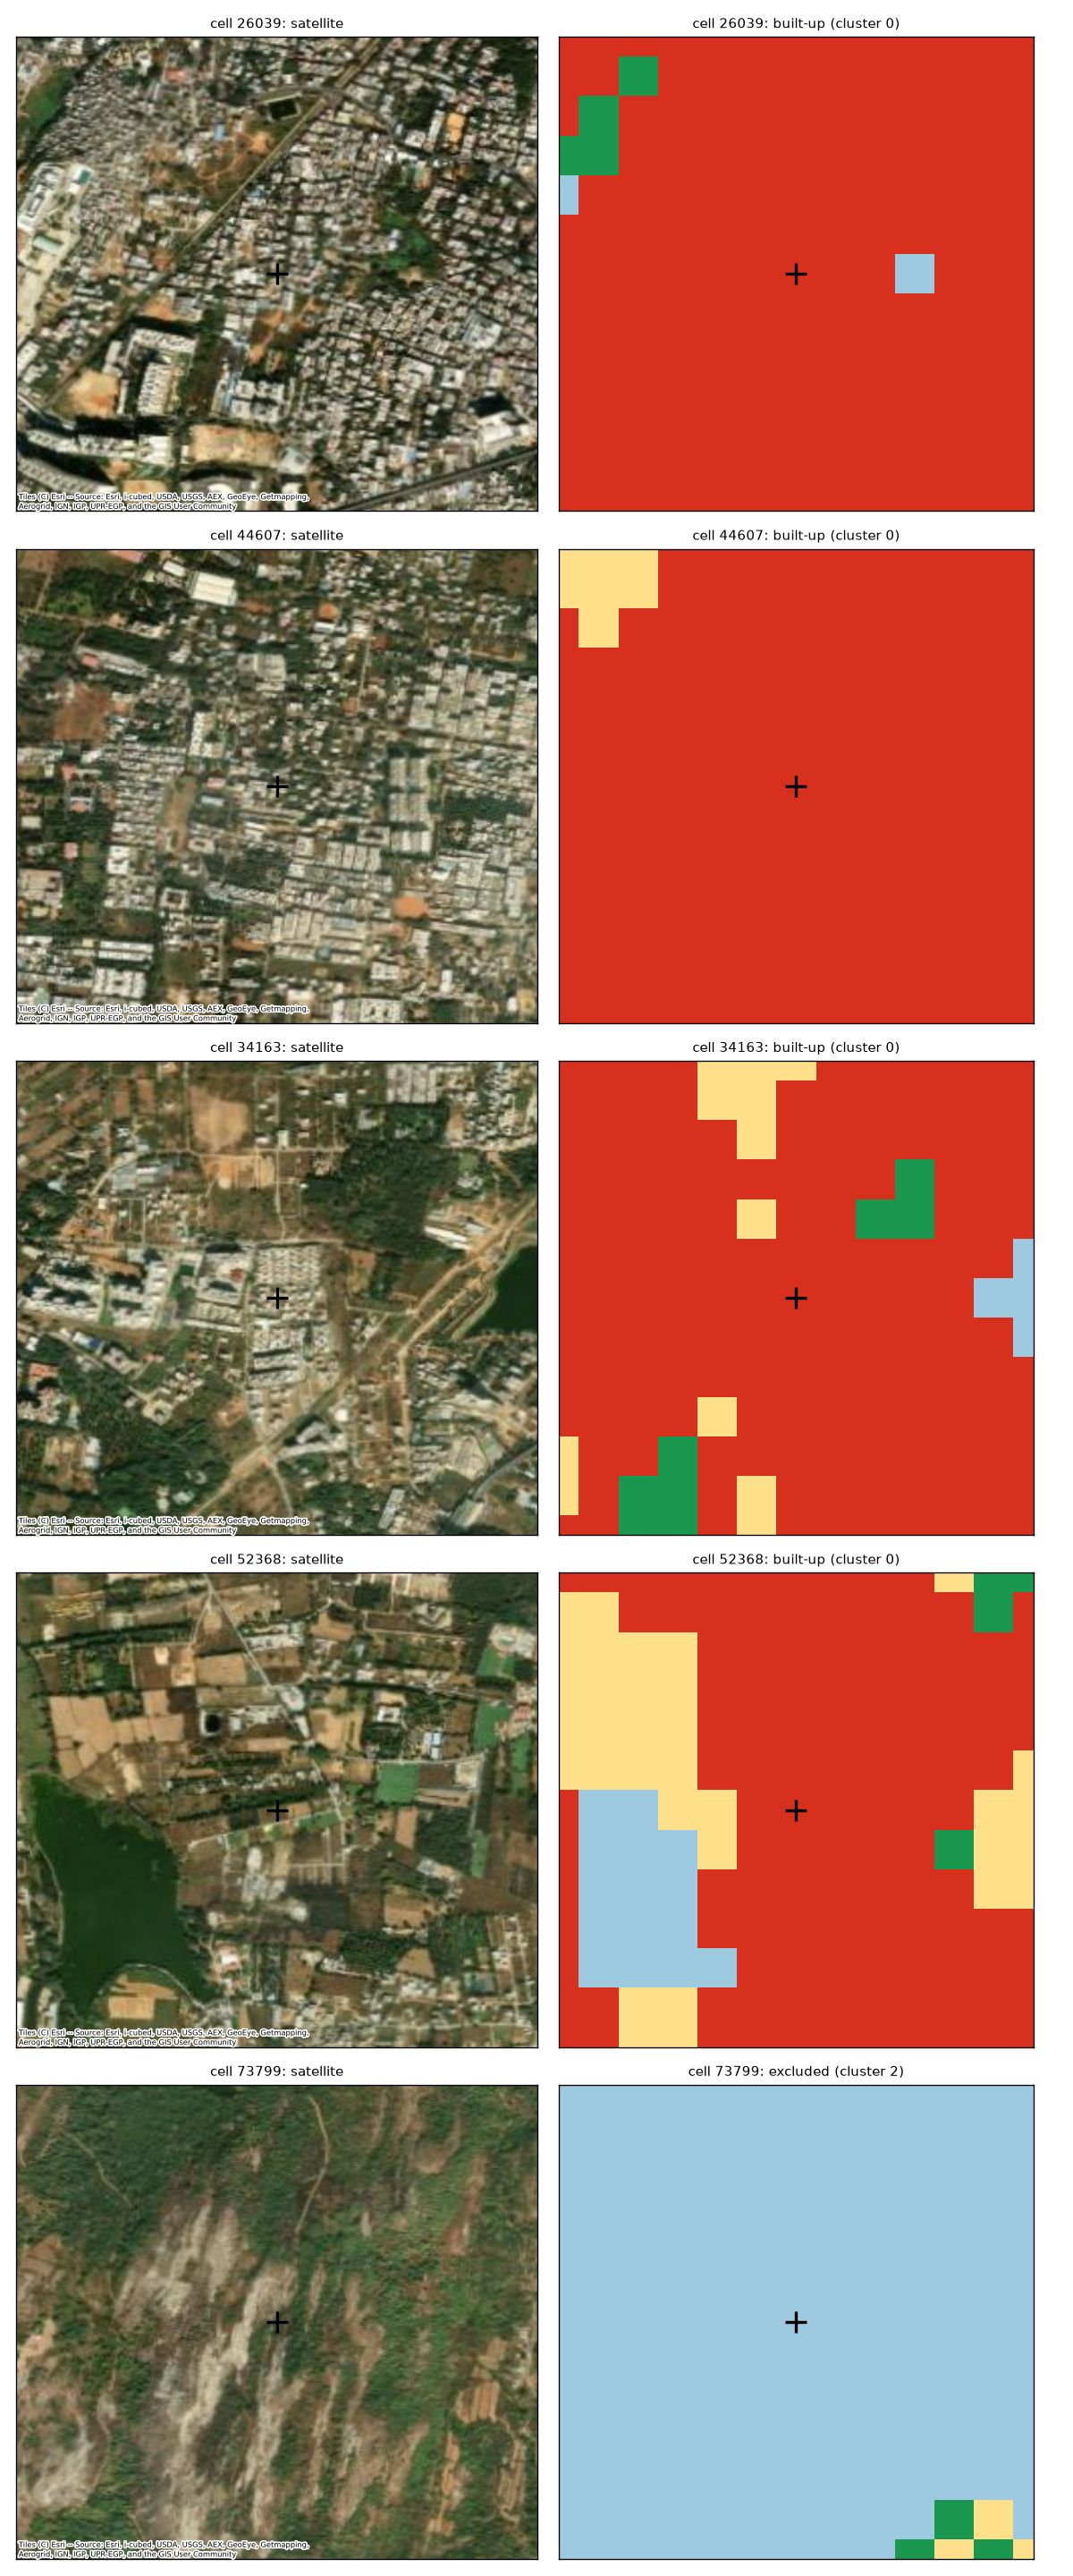
\includegraphics[height=0.86\textheight]{p5_visual_check.jpg}
\end{frame}

\end{document}
